\documentclass[12pt]{report}

\usepackage[T1]{fontenc}
\usepackage[utf8]{inputenc}
\usepackage{graphicx}
\usepackage{amsmath,amssymb,amsfonts}
\usepackage{txfonts}
\usepackage{pdfpages}
\usepackage{caption}
\usepackage{float}
\usepackage{listings}
\usepackage[polish]{babel}
\usepackage{footnote}

\makesavenoteenv{tabular}
\makesavenoteenv{table}

\renewcommand{\chaptername}{Rozdział}
\renewcommand{\contentsname}{Spis treści}
\renewcommand{\figurename}{Rys.}
\renewcommand{\tablename}{Tab.}
\renewcommand{\listfigurename}{Spis rysunków}
\renewcommand{\listtablename}{Spis tabel}
\renewcommand{\bibname}{Bibliografia}
\renewcommand\lstlistingname{Listing}
\renewcommand\lstlistlistingname{Spis listingów}

\pagestyle{headings}

\setlength{\textwidth}{14cm}
\setlength{\textheight}{20cm}

\newtheorem{definition}{Definicja}
\newtheorem{example}{Przykład}[chapter]
\newtheorem{corollary}{Wniosek}[chapter]

\begin{document}

\lstdefinelanguage{swift}
{
  morekeywords={
    func,if,then,else,for,in,while,do,switch,case,default,where,break,continue,fallthrough,return,
    typealias,struct,class,enum,protocol,var,func,let,get,set,willSet,didSet,inout,init,deinit,extension,
    subscript,prefix,operator,infix,postfix,precedence,associativity,left,right,none,convenience,dynamic,
    final,lazy,mutating,nonmutating,optional,override,required,static,unowned,safe,weak,internal,
    private,public,is,as,self,unsafe,dynamicType,true,false,nil,Type,Protocol,
  },
  morecomment=[l]{//},
  morecomment=[s]{/*}{*/},
  morestring=[b]"
}

\definecolor{keyword}{HTML}{BA2CA3}
\definecolor{string}{HTML}{D12F1B}
\definecolor{comment}{HTML}{008400}

\lstdefinestyle{customswift}{
  captionpos=b, 
  belowcaptionskip=1\baselineskip,
  breaklines=true,
  frame=LRTB,
  xleftmargin=\parindent,
  language=swift,
  showstringspaces=false,
  keywordstyle=\color{keyword},
  stringstyle=\color{string},
  commentstyle=\color{comment},
}

\lstdefinestyle{customarduino}{
  captionpos=b, 
  belowcaptionskip=1\baselineskip,
  breaklines=true,
  frame=LRTB,
  xleftmargin=\parindent,
  language=Octave,
  showstringspaces=false,
  keywordstyle=\color{keyword},
  stringstyle=\color{string},
  commentstyle=\color{comment},
}

\lstset{
  basicstyle=\ttfamily,
  showstringspaces=false,
  columns=fixed,
  keepspaces=true,
  keywordstyle=\color{keyword},
  stringstyle=\color{string},
  commentstyle=\color{comment},
  aboveskip=20pt,
  belowskip=20pt,
  numbers=left,
  firstnumber=1,
  numberfirstline=true,
  numberstyle=\ttfamily\color{gray},
}

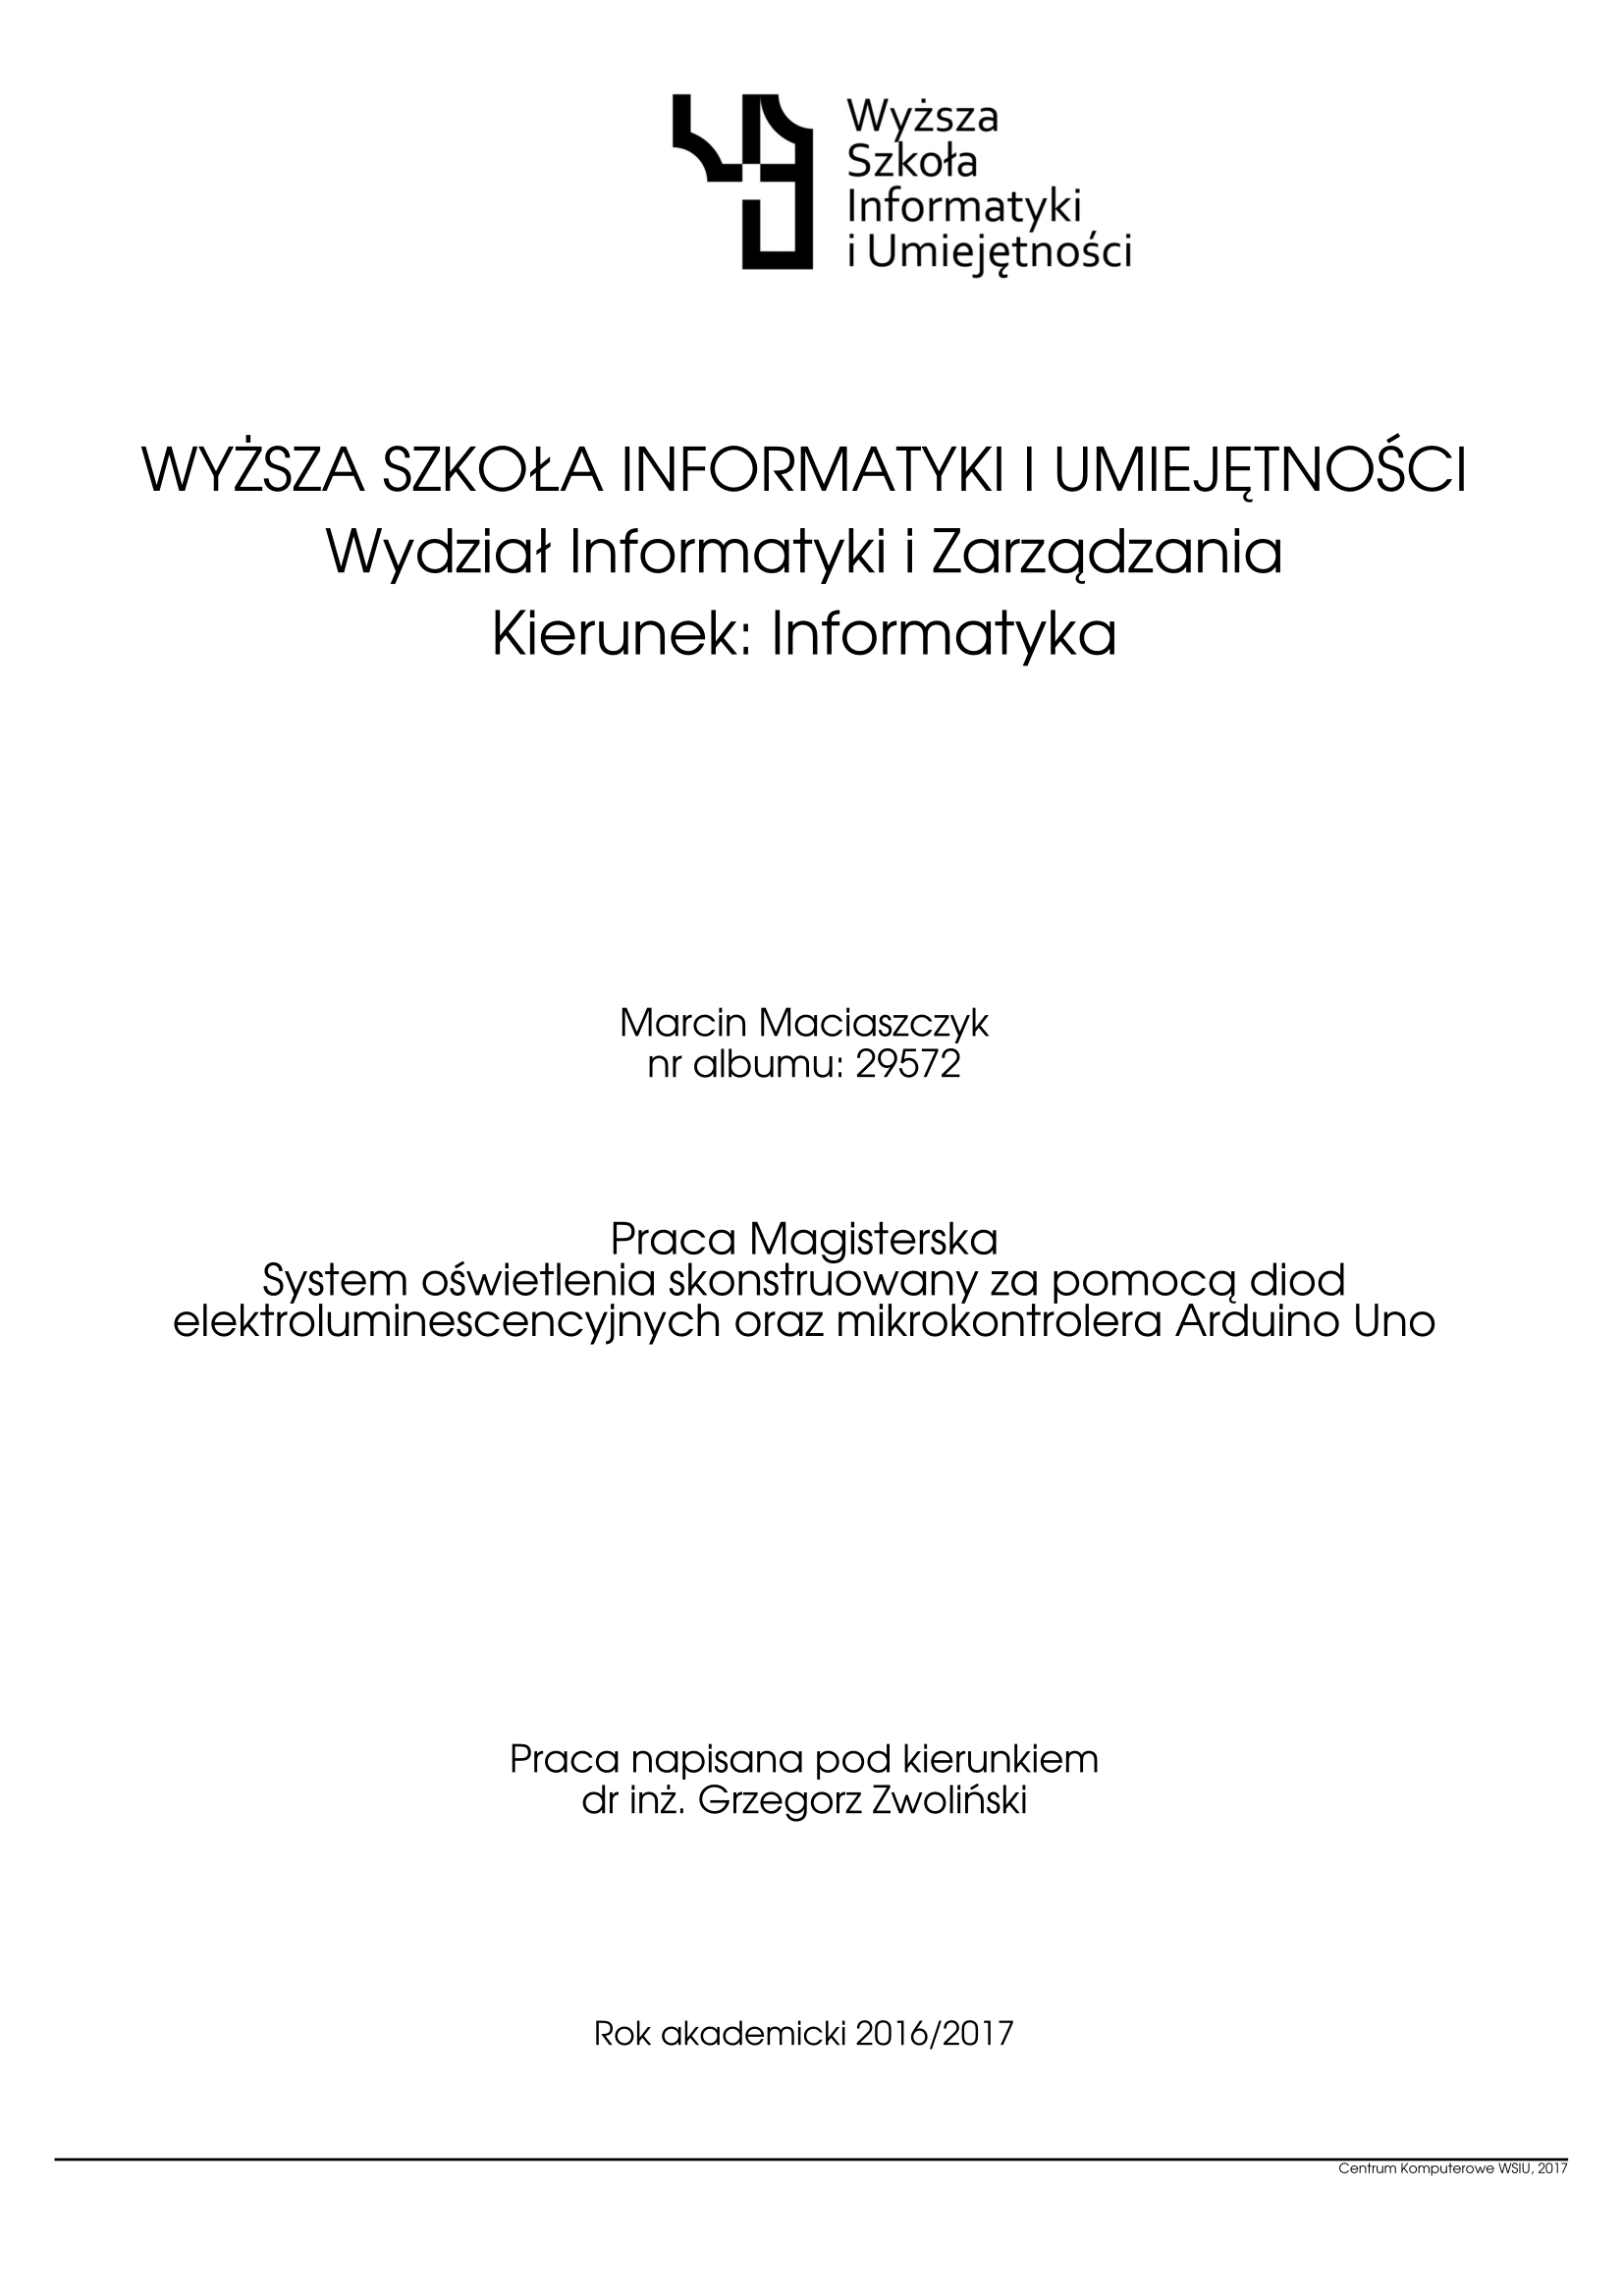
\includepdf{title-page.png}
\mbox{}
\thispagestyle{empty}
\newpage
\setcounter{page}{1}
\tableofcontents

\chapter{Wstęp}

\section{Uzasadnienie wyboru tematu}

Wraz z upływem czasu postęp technologiczny ma wpływ na życia co raz szerszej rzeszy ludzi na całym świecie. Niezliczone ilości urządzeń zagościły na stałe w~domach i mało kto wyobraża sobie bez nich swoje życie. Zaczynając od artykułów gospodarstwa domowego, a kończąc na elektronice użytkowej do której zaliczają się komputery, telewizory czy też smartfony\footnote{~Przenośne urządzenia łączące w sobie zalety telefonów komórkowych oraz przenośnych komputerów (z ang. smartphone).}. Wszystkie te urządzenia mają na~celu ułatwianie życia swoim użytkownikom.

W parze z licznymi zaletami urządzeń elektronicznych idą jednak pewne wady. Jedną z istotniejszych jest wpływ czasu spędzanego przed różnego rodzaju wyświetlaczami na zdrowie. Badania przeprowadzone na bazie danych Nielsen Audience Measurement pokazują, że przeciętny Polak spędza dziennie średnio 4,5 godziny przed ekranem telewizora\footnote{~Badania zostały przeprowadzone z uwzględnienem osób powyżej 4 roku życia w okresie od stycznia do czerwca 2015 roku \cite{czasprzedtv}.}. Nie oznacza to jednak, że przez cały ten czas ogląda on telewizję. Oglądanie filmów z dysku komputera, za pomocą serwisów VOD\footnote{~Wideo na życzenie (z ang. video on demand).} czy granie na konsoli także są wliczone w ten czas. Gdyby jednak dodać do tego czas spędzony przed ekranem smartfona czy też komputera wynik byłby zapewne dwukrotnie większy.

Pogorszenie wzroku czy też wysychanie gałki ocznej są wymieniane jako naj\-częstsze skutki zbyt dużej ilości czasu spędzanego przed ekranem. Poza próbą jego ograniczenia, jedną z częstszych porad jest próba zmniejszenia kontrastu pomiędzy ekranem a jego otoczeniem.

\begin{figure}[h]
\centering
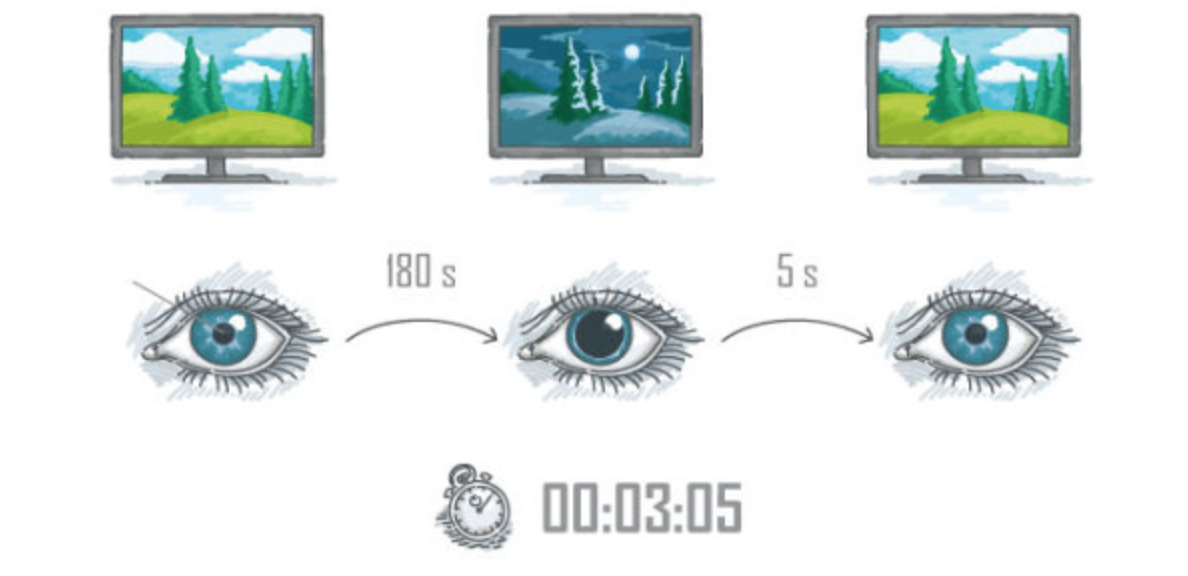
\includegraphics[width=.7\textwidth]{../resources/focuswo.png}
\caption[Średni czas dopasowania źrenicy do wyświetlanego obrazu]{Średni czas dopasowania źrenicy do wyświetlanego obrazu \cite{diagramoko}}
\end{figure}

W roku 2002 firma Philips opatentowała technologię Ambilight\footnote{~Otaczające oświetlenie (z ang. ambient lighting).}, która ma za zadanie rozszerzać obraz wyświetlany na ekranie na jego otoczenie za pomocą diod umieszczonych na tylnym panelu tworzonych telewizorów. Ambilight spotkało się z bardzo dobrym odbiorem społeczności, ponieważ poza imponującymi efektami wizualnymi zgodnie z badaniami przeprowadzonymi przez profesora Begemanna redukuje ono negatywny wpływ wyświetlaczy na oko użytkowników telewizorów~\cite{ambilightaoko}. 

\begin{figure}[h]
\centering
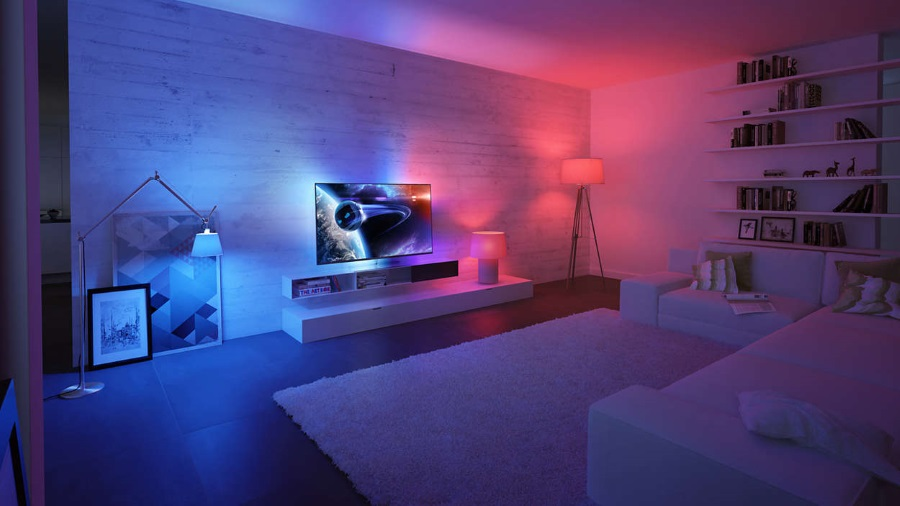
\includegraphics[width=\textwidth]{../resources/ambilight3.jpg}
\caption[Telewizor z technologią Philips Ambilight]{Telewizor z technologią Philips Ambilight \cite{ambilight2}}
\end{figure}

Ambilight posiada jednak znaczącą wadę, jest ono przeznaczone tylko dla telewizorów marki Philips, a więc nie mogą z niej korzystać użytkownicy telewizorów innych marek jak i ekranów podłączonych do komputera.

\begin{figure}[h]
\centering
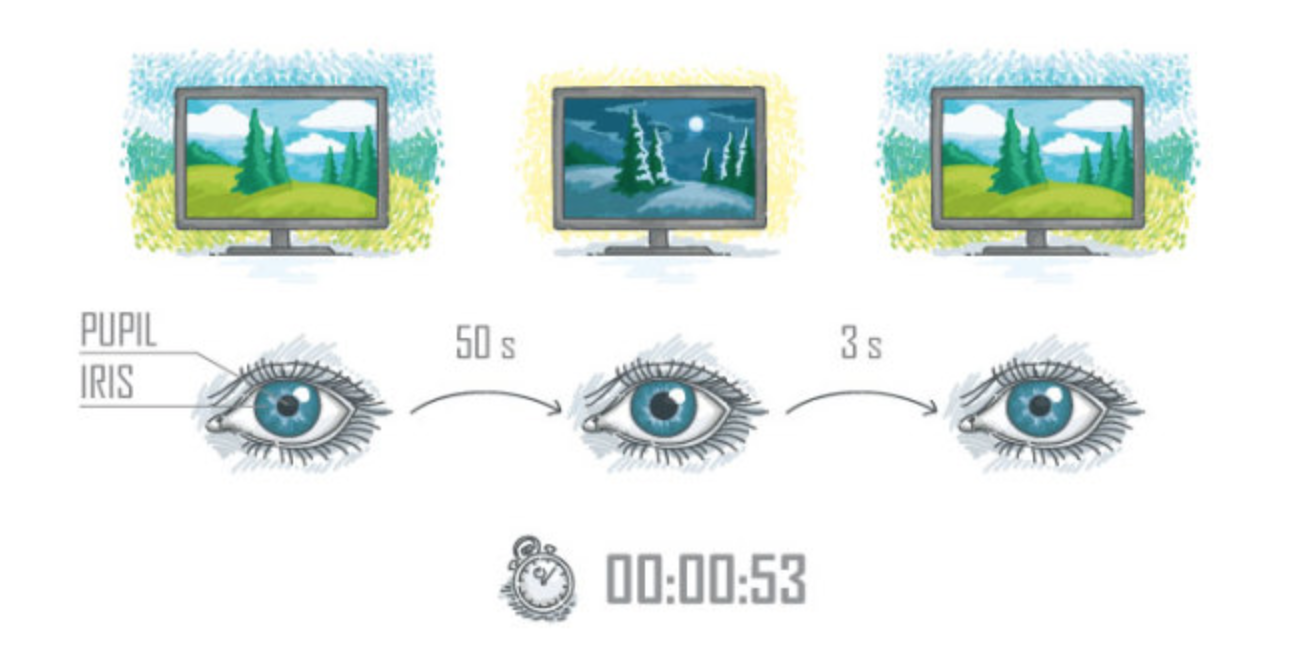
\includegraphics[width=.7\textwidth]{../resources/focusw.png}
\caption[Średni czas dopasowania źrenicy do wyświetlanego obrazu z otaczającym oświetleniem]{Średni czas dopasowania źrenicy do wyświetlanego obrazu z otaczającym oświetleniem \cite{diagramoko}}
\end{figure}

Autor niniejszej pracy jako cel postawił sobie złożenie i oprogramowanie systemu oświetlenia, który ma rozszerzać obraz widziany na ekranie na jego otoczenie w sposób podobny do Philips Ambilight. Poza zmniejszeniem kontrastu, a więc aspektem zdrowotnym, system ma także na celu zwiększyć wrażenia wizualne dostarczane przez oglądany obraz.

System oświetlenia składa się z taśmy diod elektroluminescencyjnych\footnote{~LED (z ang. light-emitting diode).} pod\-łączonych do mikrokontrolera Arduino Uno, który z kolei ma współpracować z komputerem z zainstalowanym systemem operacyjnym macOS. Oprogramowanie mikrokontrolera, którego zadaniem jest sterowanie diodami zostało przygotowane w języku Arduino, natomiast aplikacja kontrolująca cały system przeznaczona na komputer z systemem macOS została napisana w języku Swift. Wybór języków jest ściśle związany z koniecznością uzyskania jak najlepszej wydajności oraz użyciem najnowszych technologii.

Podobne systemy oświetlenia dostępne są już od pewnego czasu na rynku, jednak to właśnie nowoczesne technologie, prostota wykonania i niskie koszta powinny uczynić z Ligtning, bo taką nazwę otrzymał projekt, pełnowartościowego konkurenta.

\section{Problematyka i zakres pracy}

Różnego rodzaju wyświetlacze towarzyszą w dniu codziennym większości ludzi. Co raz większa jest także popularność różnego rodzaju gadżetów elektronicznych. Niektórzy decydują się nawet na budowanie własnych narzędzi wykorzystując gotowe komponenty takie jak mikrokontrolery i inne urządzenia peryferyjne. Niniejsza praca porusza właśnie problematykę tworzenia oprogramowania przeznaczonego komputer jak i mikrokontroler, którego zadaniem będzie sterowanie taśmą diod elektroluminescencyjnych.

Zadanie to wymaga przejścia kilku kolejnych etapów, które składają się na zakres pracy:

\begin{enumerate}
	\item Analiza istniejących rozwiązań realizujących podobne zadania.
	\item Zebranie wymagań umożliwiających stworzenie konkurencyjnego systemu oświeletnia.
	\item Zaprojektowanie systemu oświetlenia.
	\item Skompletowanie odpowiednich komponentów i ich podłączenie.
	\item Zaprojektowanie oprogramowania systemu oświetlenia przeznaczonego na mikrokontroler i komputer.
	\item Implementacja oprogramowania.
	\item Dokumentacja projektu.
	\item Analiza stworzonego systemu oświetlenia.
	\item Dyskusja osiągniętych wyników jak i perspektywy rozwoju projektu.
\end{enumerate}

\section{Cele pracy}

Do najważniejszych celów niniejszej pracy dyplomowej należą:

\begin{itemize}
	\item Analiza istniejących systemów oświetlenia o podobnym działaniu, a co za tym idzie dokładniejsze zapoznanie się z istniejącymi rozwiązaniami. Umożliwiło to sprecyzowanie wymagań oraz podjęcie kluczowych decyzji do\-tyczą\-cych wykorzystanych komponentów czy też technologii.
	\item Stworzenie własnego systemu oświetlenia umożliwiające dokładne zapoznanie się problematyką projektu, czyli między innymi:
	\begin{itemize}
		\item Tworzeniem wielomodułowych systemów, a więc synchronizacji i komunikacji pomiędzy modułami.
		\item Kompletowaniem złożonego z kilku komponentów systemu oświetlenia.
		\item Optymalizacją obliczeń związanych z przechwytywaniem i obróbką obrazu.
		\item Projektowaniem graficznego interfejsu użytkownika.
	\end{itemize}
	\item Porównanie Lightning z analizowanymi wcześniej systemami mające na celu stwierdzić czy przyjęte założenia i wymagania okazały się trafne.
\end{itemize}

\section{Metoda badawcza}

\subsection{Studia literaturowe}

Większość źródeł odnoszących się do tematyki niniejszej pracy znajduje się w Internecie. Źródła te można podzielić na następujące kategorie:

\begin{itemize}
	\item Tworzenie oprogramowania w języku Swift.
	\item Tworzenie oprogramowania przeznaczonego na mikrokontroler Arduino.
	\item Zagadnienia związane z mikrokontrolerami.
\end{itemize}

Rozdział  \ref{literatura} przedstawia najważniejsze pozycje spośród z każdej wymienionych kategorii źródeł.

\subsection{Analiza istniejących systemów oświetlenia}

Studia literaturowe to jedna z ważniejszych metod badawczych, jednakże analiza istniejących systemów oświetlenia jest równie istotna. Umożliwia ona wczesne zlokalizowanie istniejących problemów związanych z wybraną tematyką jak, braków istniejących rozwiązań i sprecyzowanie potrzeb użytkowników.

\subsection{Stworzenie własnego systemu oświetlenia}

Etapem następnym po zapoznaniu się z istniejącą literaturą i przeprowadzeniu analizy istniejących systemów oświetlenia jest stworzenie właśnego systemu oświetlenia. Jest to ważna metoda badawcza,
ponieważ umożliwia dogłębne zapoznanie się z problematyką pracy jak i przejście przez wszystkie etapy tworzenia własnego systemu wykorzystującego mikrokontroler Arduino współpracujący z komputerem. Wszystkie napotkane problemy muszą zostać rozwiązane w jak najbardziej optymalny sposób, prowadzi to więc to do precyzyjnego zbadania wybranej tematyki.

\subsection{Analiza porównawcza oraz testy}

Analiza stworzonego systemu oświetlenia i porównanie go z isniejącymi już rozwią\-zaniami ma za zadanie poprowadzić do jak najtrafniejszych wniosków. Celem tego etapu jest dowiedzenie się czy przyjęte założenia i wybrane rozwiązania są lepsze od tych które przyjęli autorzy istniejących już rozwiązań.

\section{Przegląd literatury w dziedzinie} \label{literatura}

\subsection{Tworzenie oprogramowania w języku Swift}

Swift został opublikowany przez Apple w 2014 roku. Jest on następcą języka znanego jako Objective C, posiada on szereg usprawnień i nowych funkcjonalności mających za zadanie sprawić aby tworzenie oprogramowania na platforme Mac było jeszcze sprawniejsze. Oto lista wykorzystanych źródeł, które są związane z właśnie tym językiem:

\begin{itemize}
	\item {\it The Swift Programming Language (Swift 3.1)} \cite{swiftpub} -- Najlepsze i najdokładniejsze źródło informacji dotyczących Swifta. Publikacja utworzona przez twórców języka, firmę Apple.
	\item {\it App Development with Swift} \cite{swiftdev} -- Kurs nauki programowania w języku Swift utworzony przez firmę Apple.
	\item Oficjalna strona internetowa otwartoźródłowego projektu Swift \cite{swiftstr} -- Źródła, przydatne projekty oraz przede wszystkim odnośniki do dokumentacji.
	\item Strona Apple Developer \cite{swiftapple} -- Obszerna baza gotowych przykładów, dokumentacja oraz pomoce dotyczące środowiska Xcode.
\end{itemize}

Fakt, że są to jedynie źródła internetowe związany jest głównie z niskim wiekiem języka a także jego ciągłym rozwojem.

\subsection{Tworzenie oprogramowania przeznaczonego na mikrokontroler Arduino}

% TODO TODO TODO TODO TODO TODO TODO TODO TODO TODO TODO TODO TODO TODO TODO
% TODO TODO TODO TODO TODO TODO TODO TODO TODO TODO TODO TODO TODO TODO TODO
% TODO TODO TODO TODO TODO TODO TODO TODO TODO TODO TODO TODO TODO TODO TODO

\subsection{Zagadnienia związane z mikrokontrolerami}

% TODO

\section{Układ pracy}

Temat niniejszej pracy to system oświetlenia skonstruowany za pomocą diod elektroluminescencyjnych oraz mikrokontrolera Arduino Uno. Jej głównym celem jest przeanalizowanie istniejących systemów oświetlenia oraz stworzenie własnego ro\-związania.

Praca rozpoczyna się od uzasadnienia wyboru tematu pracy, a także opisu celów pracy, jej problematyki, zakresu, wykorzystanych metod badawczych, przeglądu literatury oraz jej układu.

W kolejnym rozdziale zawarte zostały objaśnienia zagadnień teoretycznych po\-wiązanych z tematyką pracy.

Następnie przeanalizowano istniejące już systemy oświetlenia biorąc pod uwagę wcześniej zdefiniowane kryteria.

Kolejny rozdział opisuje projekt systemu oświetlenia Lightning tworzonego w ramach części badawczej niniejszej pracy. W rozdziale tym opisane zostają wymagania postawione przed projektem, komponenty z jakich będzie się on składał, tworzone moduły oprogramowania, diagram klas projektu, wykorzystane wzorce projektowe czy też sama implementacja. Rozdział kończy analiza wykonanego projektu i jego dokumentacja w postaci podręcznika użytkownika, opisu dodawania własnych animacji i perspektyw rozwoju projektu.

Pracę kończy podsumowanie, które zawiera dyskusję wyników oraz dalsze prespektywy jej rozwoju.

\chapter[Zagadnienia teoretyczne]{Zagadnienia teoretyczne}

% TODO protokoly, swift, port szereg, przechtywywanie obrazu, mikrokontrolery

\chapter[Analiza istniejących rozwiązań]{Analiza istniejących rozwiązań}

\section{Kryteria analizy} \label{kryt}

Tak jak to zostało wspomniane na wstępie projektowany system oświetlenia nie jest pierwszym w swoim rodzaju i ma on do czynienia ze sporą konkurencją w postaci istniejących już rozwiązań. W rozdziale tym zostanie przeprowadzona ich analiza, jednak przed przystąpieniem do niej konieczne jest zdefiniowanie kryteriów jakie zostaną wzięte pod uwagę. Kryteria te powinny mieć pokrycie z oczekiwaniami użytkowników, a Lightning powinno wyróżniać się co najmniej pod paroma względami. Po zapoznaniu się z opiniami użytkowników w Internecie pod uwagę zostały wzięte następujące kryteria:

\begin{itemize}
	\item Koszt -- Dla większości potencjalnych użytkowników może to być kluczowe kryterium wyboru, dlatego koszt zakupu gotowego systemu lub koszt skompletowania komponentów powinien być jak najniższy.
	\item Rodzaj systemu -- Najwyżej cenione są systemy zintegrowane z wyświetlaczami, gotowe do uruchomienia od razu po zakupie. Im trudniejsze jest skompletowanie systemu oraz oprogramowanie tym mniej użytkowników z niego skorzysta.
	\item Płynność działania -- Tylko systemy działające płynnie są w stanie zatrzymać przy sobie swoich użytkowników.
	\item Możliwość konfiguracji -- Sprawia, że każdy może dopasować system do siebie, im większa tym lepiej.
	\item Interfejs użytkownika -- Rzecz na którą wielu użytkowników zwraca uwagę na początku, im bardziej przejrzysty i łatwy z obsłudze tym lepiej.
	\item Dodatkowe możliwości -- Bonusy takie jak tryb animacji czy wizualizacji odtwarzanej muzyki wpływają na powiększenie oceny końcowej.
	\item Wspierany sprzęt i oprogramowanie -- Wsparcie dla różnego rodzaju platform i systemów operacyjnych zwiększa grono potencjalnych odbiorców.
	\item Licencja -- Rodzaj licencji na jakiej udostępniane jest oprogramowanie ma znaczenie w licznych przypadkach. Większość użytkowników postawiona przed wyborem pomiędzy restrykcyjną licencją a oprogramowaniem otwarto-źródłowym wybierze to drugie.
\end{itemize} 

\section{Porównanie istniejących rozwiązań} \label{por}

\subsection{Technologia Philips Ambilight}

Pierwsze miejsce w zestawieniu istniejących rozwiązań zajmuje technologia Ambilight opatentowana w 2002 roku przez firmę Philips. Pierwszy telewizor z Ambilight trafił do sklepów w 2004 roku. W chwili obecnej dostępnych jest dużo więcej modeli wyposażonych w Ambilight, który cieszy się sporą popularnością.

\begin{figure}[h]
\centering

\includegraphics[width=.7\textwidth]{../resources/ambilight.jpg}
\caption[Logo Philips Ambilight]{Logo Philips Ambilight \cite{ambilight}}
\end{figure}

\newpage

\begin{table}[h]
\centering
\begin{tabular}{| l | l |} 
\hline 
Koszt & \\ \hline
Rodzaj systemu & gotowy do użycia, zintegrowany \\ \hline
Płynność działania & bardzo wysoka \\ \hline
Możliwość konfiguracji & duża  \\ \hline
Interfejs użytkownika & intuicyjny  \\ \hline
Dodatkowe możliwości &  obsługa dodatkowych lamp, \\ \hline
&  aplikacja mobilna \\ \hline
Wspierany sprzęt i oprogramowanie &  tylko telewizory marki Philips   \\ \hline
Licencja & opatentowana technologia,  \\ \hline
& brak dostępu do źródeł  \\ \hline
\end{tabular} 
\caption{Analiza technologii Philips Ambilight}
\end{table}

\begin{figure}[h]
\centering
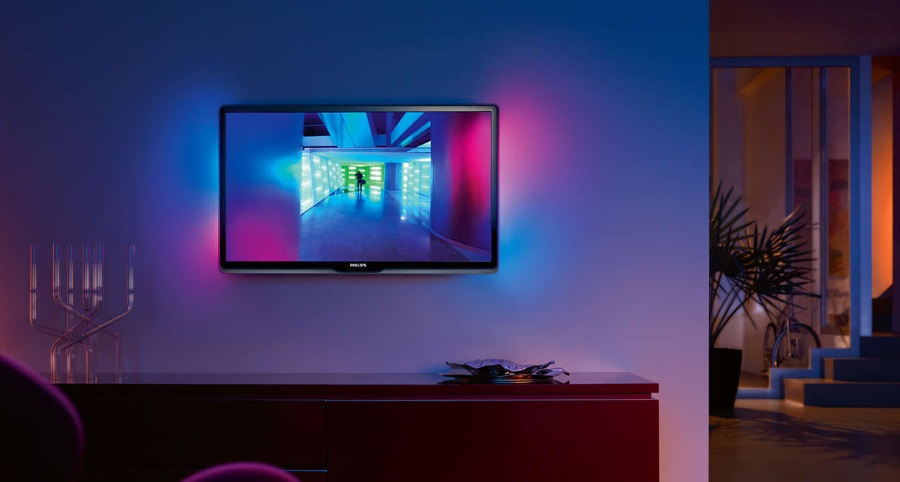
\includegraphics[width=\textwidth]{../resources/ambilight2.jpg}
\caption[Telewizor z technologią Philips Ambilight]{Telewizor z technologią Philips Ambilight \cite{ambilight2}}
\end{figure}

Do największych zalet technologii Ambilight należy jej integracja z telewizorami Philips. Dzięki temu działa płynnie, ma duże możliwości konfiguracyjne, intuicyjny interfejs a także inne dodatkowe możliwości. Wielu użytkowników doceni też brak konieczności podłączania dodatkowych urządzeń zewnętrznych. Część z nich uzna to za wadę, bo systemu oświetlenia nie da się przenieść do innego wyświetlacza.

Do wad Ambilight zaliczyć można wysoki koszt, wsparcie jedynie dla telewizorów marki Philips a także restrykcyjną licencję.

% TODO koszt i link do źródła informacji

\subsection{System oświetlenia Lightpack} \label{lightpack}

Kolejne miejsce w zestawieniu zajmuje system oświetlenia Lightpack. Jest to projekt ufundowany przez społeczność\footnote{~ Z ang. crowd-funding.} za pomocą serwisu Kickstarter \cite{lpk}, gdzie zebrał ponad pół miliona dolarów.

\begin{figure}[h]
\centering
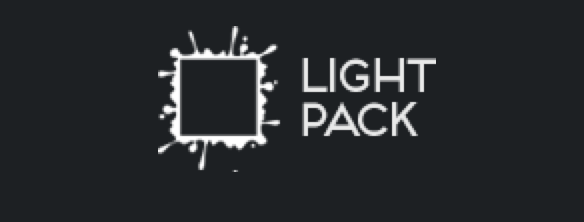
\includegraphics[width=.7\textwidth]{../resources/lightpack.png}
\caption[Logo Lightpack]{Logo Lightpack \cite{lps}}
\end{figure}

\begin{table}[h]
\centering
\begin{tabular}{| l | l |} 
\hline 
Koszt & od 119 dolarów, czyli około 482 zł \\ \hline
Rodzaj systemu & gotowy do użycia, zewnętrzny \\ \hline
Płynność działania & wysoka \\ \hline
Możliwość konfiguracji & duża  \\ \hline
Interfejs użytkownika & intuicyjny  \\ \hline
Dodatkowe możliwości &  animacja przejść pomiędzy kolorami, \\ \hline
& pełna konfiguracja obszarów diod \\ \hline
Wspierany sprzęt i oprogramowanie &  dowolny komputer i telewizor   \\ \hline
Licencja & kod otwartoźródłowy  \\ \hline
\end{tabular} 
\caption{Analiza systemu oświetlenia Lightpack}
\end{table}

Nawiększą zaletą Lightpack jest multiplatformowość, działa on z każdym telewizorem oraz komputerami z systemami Windows, Linux jak i macOS. Posiada on także spore możliwości konfiguracyjne. Otwartoźródłowy kod również zalicza się do zalet, choć kod znajdujący się na repozytorium nie jest już uaktualniany od długiego czasu \cite{legacy}.

Minusem jest dość wysoka cena jak i konieczność podłączenia dodatkowego urządzenia do wyświetlacza. Diody montowane są za pomocą samoprzypelnych taśm co również nie musi spodobać się wszystkim użytkownikom.

\begin{figure}[h]
\centering
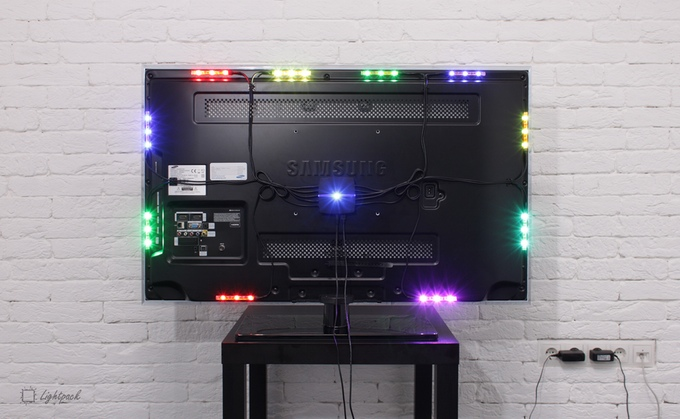
\includegraphics[width=\textwidth]{../resources/lightpackm.jpg}
\caption[Telewizor z systemem oświetlenia Lightpack]{Telewizor z systemem oświetlenia Lightpack \cite{lps}}
\end{figure}

\begin{figure}[h]
\centering
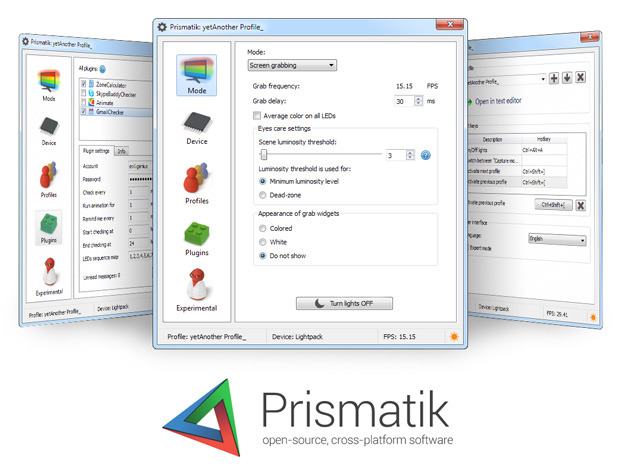
\includegraphics[width=.8\textwidth]{../resources/prismatik.jpg}
\caption[Aplikacja sterująca systemu oświetlenia Lightpack]{Aplikacja sterująca systemu oświetlenia Lightpack \cite{lps}}
\end{figure}

\vfill
\clearpage

\subsection{System oświetlenia Lightpack 2}

Lightpack 2 jest kontynuacją opisanego w rozdziale \ref{lightpack} projektu Lightpack. Wprowadza on jednak sporo zmian i podobnie jak swój poprzednik został ufundowany z wykorzystaniem serwisu Kickstarter \cite{lp2k}, gdzie również zebrał ponad pół miliona dolarów.

\begin{figure}[h]
\centering
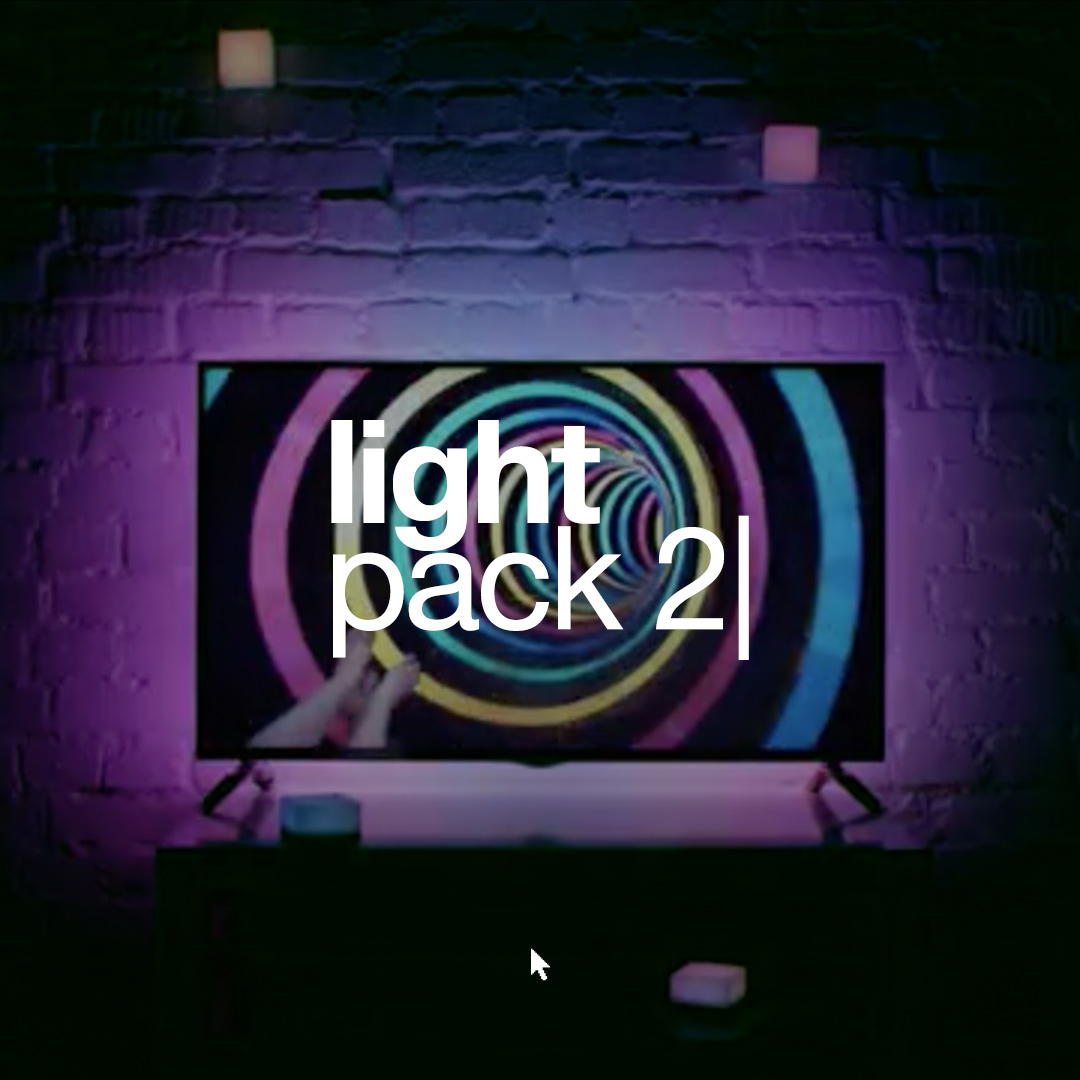
\includegraphics[width=.5\textwidth]{../resources/lightpack2.jpg}
\caption[Logo Lightpack 2]{Logo Lightpack 2 \cite{lp2s}}
\end{figure}

\begin{table}[h]
\centering
\begin{tabular}{| l | l |} 
\hline 
Koszt & od 239 dolarów, czyli około 968 zł \\ \hline
Rodzaj systemu & gotowy do użycia, zewnętrzny \\ \hline
Płynność działania & wysoka \\ \hline
Możliwość konfiguracji & bardzo duża  \\ \hline
Interfejs użytkownika & intuicyjny  \\ \hline
Dodatkowe możliwości &  animacja przejść pomiędzy kolorami, \\ \hline
& pełna konfiguracja obszarów diod, \\ \hline
& aplikacja mobilna, dodatkowe lampy \\ \hline
Wspierany sprzęt i oprogramowanie &  dowolny komputer i telewizor   \\ \hline
Licencja & brak dostępu do źródeł,  \\ \hline
& dostępne stare źródła aplikacji sterującej \\ \hline
\end{tabular} 
\caption{Analiza systemu oświetlenia Lightpack 2}
\end{table}

System Lighpack 2 posiada zalety swojego poprzednika, jednak dodaje on zupełnie nowe możliwości. Ciekawym dodatkiem jest obsługa zewnętrznych lamp rozmieszczonych w tym samym pomieszczeniu co wyświetlacz. Dodano aplikację mobilną. Najważniejszy jest jednak fakt, że nie wymaga on połączenia z komputerem. Tym razem podłączany on jest do dowolnego źródła sygnału HDMI, w tym konsoli czy dekodera telewizyjnego.

Dużą wadą systemu jest spora cena, która rośnie wraz z chęcią dokupienia dodatkowych lamp czy też większej ilościo diod. Ponadto na Lighpack 2 trzeba jeszcze poczekać, ponieważ jest on w ostatniej fazie produkcji i na razie możliwe jest jedynie składanie zamówień.

\begin{figure}[h]
\centering
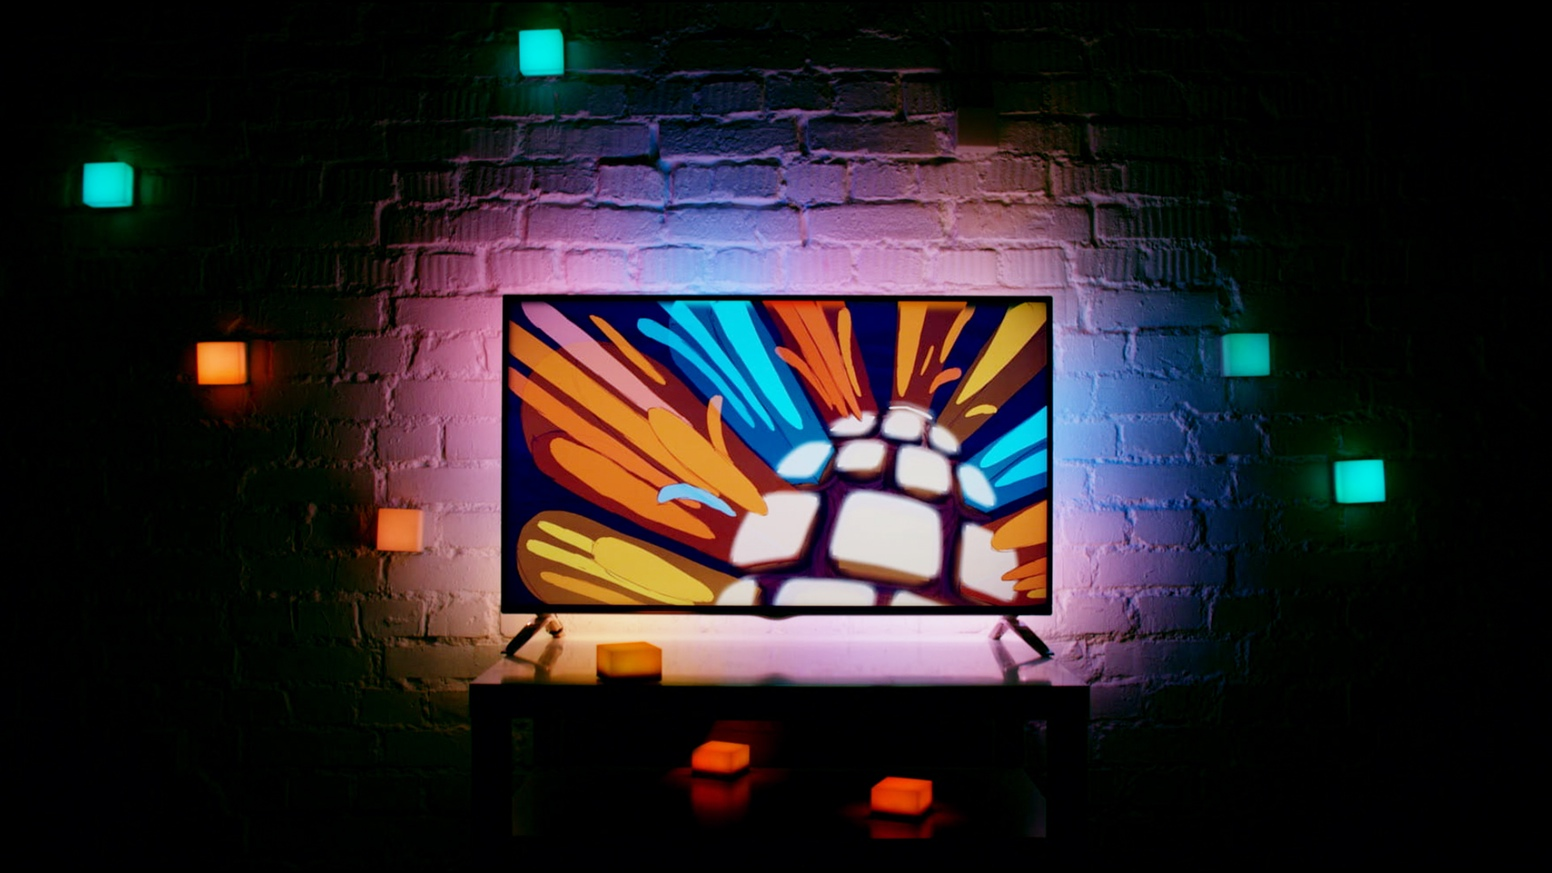
\includegraphics[width=\textwidth]{../resources/lightpack2m.jpg}
\caption[Telewizor z systemem oświetlenia Lightpack 2]{Telewizor z systemem oświetlenia Lightpack 2 \cite{lp2s}}
\end{figure}

\chapter{System oświetlenia Lightning}

\section{Analiza wymagań}

\subsection{Wymagania funkcjonalne}

W celu stworzenia jak najatrakcyjniejszego system oświetlenia podczas projektowania Lightning przyjęto poniższe wymagania funkcjonalne:

\begin{itemize}
\item System musi udostępniać tryb przechwytywania rozszerzający obraz wyświetlany na ekranie na jego otoczenie za pomocą diod elektroluminescencyjnych.
\item System musi posiadać tryb animacji. Powinien być on łatwy do rozszerzenia o kolejne animacje.
\item System musi być konfigurowalny z poziomu aplikacji sterującej. Konfiguracji podlegać musi co najmniej liczba i rozmieszczenie diod za ekranem, a także wykorzystywany port szeregowy.
\item Projekt musi być odpowiednio udokumentowany. Dokumentacja powinna ułatwiać szybkie skonfigurowanie oraz uruchomienie systemu.
\end{itemize}

\subsection{Wymagania niefunkcjonalne}

Do wymagań niefunkcjonalnych postawionych przed projektowanym systemem należą:

\begin{itemize}
\item System musi działać płynnie, a więc liczba osiąganych klatek na sekundę powinna być jak największa nawet przy dużych rozdzielczościach przechwytywanego ekranu.
\item Korzystanie z aplikacji sterującej powinno być jak najbardziej intuicyjne, a użytkownik powinien mieć dostęp do wskazówek dotyczących jej interfejsu.
\item Oprogramowanie mikrokontrolera powinno oferować jak najprostszy interfejs i zawierać jak najmniej logiki sterującej.
\item Pamięć na obu urządzeniach sterujących powinna być odpowiednio zarządzana, niedopuszczalne są wycieki pamięci czy też zapętlenia programu.
\end{itemize}

\section{Komponenty systemu} \label{komp}

Do konstrukcji systemu wykorzystane zostały następujące komponenty:

\begin{itemize}
	\item Cyfrowo adresowany łańcuch składający się z 25 diod elektroluminescencyjnych o średnicy 12 mm ze sterownikiem WS2801. Dostępny w sklepie internetowym Botland w cenie 195 zł \cite{diody}.
	\item Stabilizowany zasilacz sieciowy o napięciu wyjściowym 5 V. Dostępny w sklepie internetowym Botland w cenie 19,90 zł \cite{zasilacz}.
	\item Wtyk ze złączem pozawalającym połączyć łańcuch z zasilaczem. Dostępny w sklepie Botland w cenie 1,90 zł \cite{wtyk}.
	\item Mikrokontroler Arduino Uno w wersji 3. Dostępny w sklepie Botland w cenie 95 zł \cite{arduino}.
	\item Przewód USB. Dostępny w sklepie Botland w cenie 4,90 zł \cite{usb}.
\end{itemize}

Łańcuch z diodami został podłączony od jednej strony za pomocą wymienionego wcześniej wtyku z zasilaczem, z drugiej strony natomiast z mikrokontrolerem. Ten z kolei komunikuje się z komputerem z systemem macOS za pomocą przewodu USB. Dokładny schemat połączenia komponentów przedstawia rysunek \ref{schemat}.
	
\begin{figure}[h]
\centering
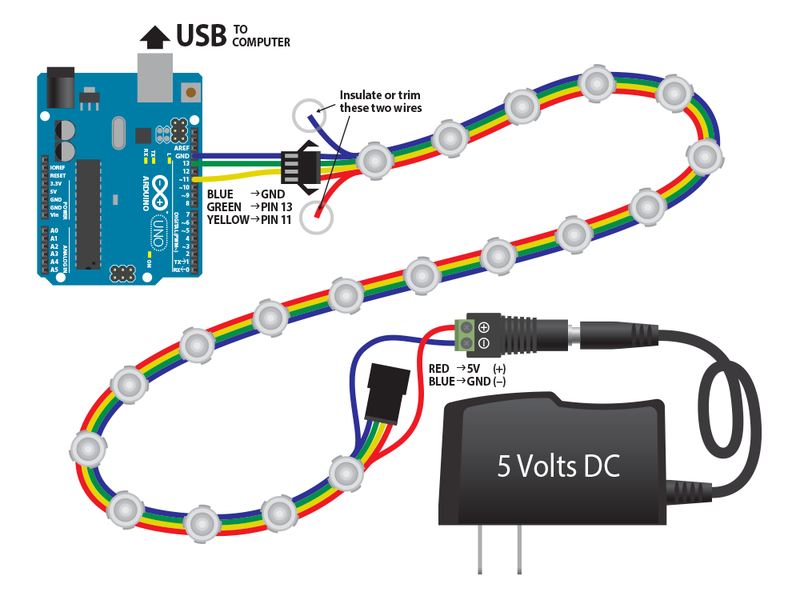
\includegraphics[width=\textwidth]{../resources/wiring.png}
\caption[Schemat podłączenia komponentów systemu]{Schemat podłączenia komponentów systemu \cite{schemat}}
\label{schemat}
\end{figure}
		
Koszt związany ze skompletowaniem wszystkich komponentów wyniósł łącznie 316,70 zł. Cena ta mogłaby ulec znacznemu zmniejszeniu w przypadku użycia kompatybilnych zamienników dla najdroższych elementów, czyli dla łańcucha diod czy też Arduino Uno w najnowszej wersji. Ponadto komponenty te mogą zostać wykorzystane w innych systemach.

% TODO opis oraz zdjęcie mocowania diod

\section{Moduły oprogramowania}

\subsection{Oprogramowanie mikrokontrolera}

Głównym celem oprogramowania przeznaczonego na mikrokontroler jest zarządza\-nie diodami. Dzieje się to w oparciu o polecenia otrzymywane portem szeregowym od komputera, który steruje całym systemem. W związku z charakterem swojego zadania oprogramowanie musi działać jak najszybciej oraz posiadać jak najmniej logiki sterującej. Kontrola diod ogranicza się do przesyłania pakietów danych otrzymywanych z komputera na odpowiednie wyjścia do których diody są podłączone do mikrokontrolera. 

Moduł ten został napisany w natywnym języku Arduino, który udostępnia wszystkie podstawowe funkcje umożliwiające stworzenie oprogramowania spełniającego postawione przed nim wymagania.

\subsection{Aplikacja przeznaczona na komputer}

W przeciwieństwie do swojego poprzednika moduł przeznaczony na komputer ma za zadanie sterowanie całym systemem. Odpowiada on bezpośrednio na żądania użytkownika wydawane za pomocą stworzonego interfejsu graficznego i komunikuje się z oprogramowaniem mikrokontrolera w celu przekazania instrukcji zapalenia pewnej konfiguracji diod. Komunikacja odbywa się nieprzerwanie, jednokierunkowo, a każdy pakiet jest poprzedzony nagłówkiem składającym się z 11 bajtów.

Aplikacja ta może działać w dwóch trybach:

\begin{itemize}
	\item Tryb przechwytywania w którym przechwytywany jest obraz wybranego wyświetlacza, a każda dioda świeci się w kolorze odpowiadającego jej koloru ekranu. W trybie tym użytkownik powinien mieć kontrolę nad jasnością diod a także możliwość wygładzania przejść aby uniknąć szybkich zmian kolorów.
	\item Tryb animacji w którym za pomocą diod system wyświetla przygotowane wcześniej animacje. Animacje zapisane są jako klasy w języku Swift. Użytkownik poza wyborem animacji ma wpływ na użyte w niej kolory oraz prędkość animacji.
\end{itemize}

Ponadto aplikacja posiada możliwość konfiguracji liczby i rozmieszczenia diod, a także wykorzystywanego portu szeregowego.
Aplikacja została napisana w języku Swift, który jest przeznaczony dla komputerów z systemem macOS. Umożliwia on szybkie projektowanie interfejsów graficznych zgodnych z wyglądem systemu oraz przede wszystkim udostępnia on wszystkie podstawowe funkcje obiektowego języka programowania co jest istotne podczas projektowania aplikacji, której logika nie jest już tak prosta jak w przypadku oprogramowania mikrokontrolera.

\section{Projekt}

\subsection{System kontroli wersji}

Podczas pracy nad projektami programistycznymi często wymagana jest współpraca kilku programistów, cofanie pomyłkowo wprowadzonych zmian czy też dziennik zadań do wykonania. Wspomniane funkcjonalności udostępniają systemy kontroli wersji. Do najpopularniejszych należy Git, którego funkcjonalność darmowo udostępnia serwis   GitHub, gdzie z kolei znajduje się repozytorium projektu \cite{github}.

\begin{figure}[h]
\centering
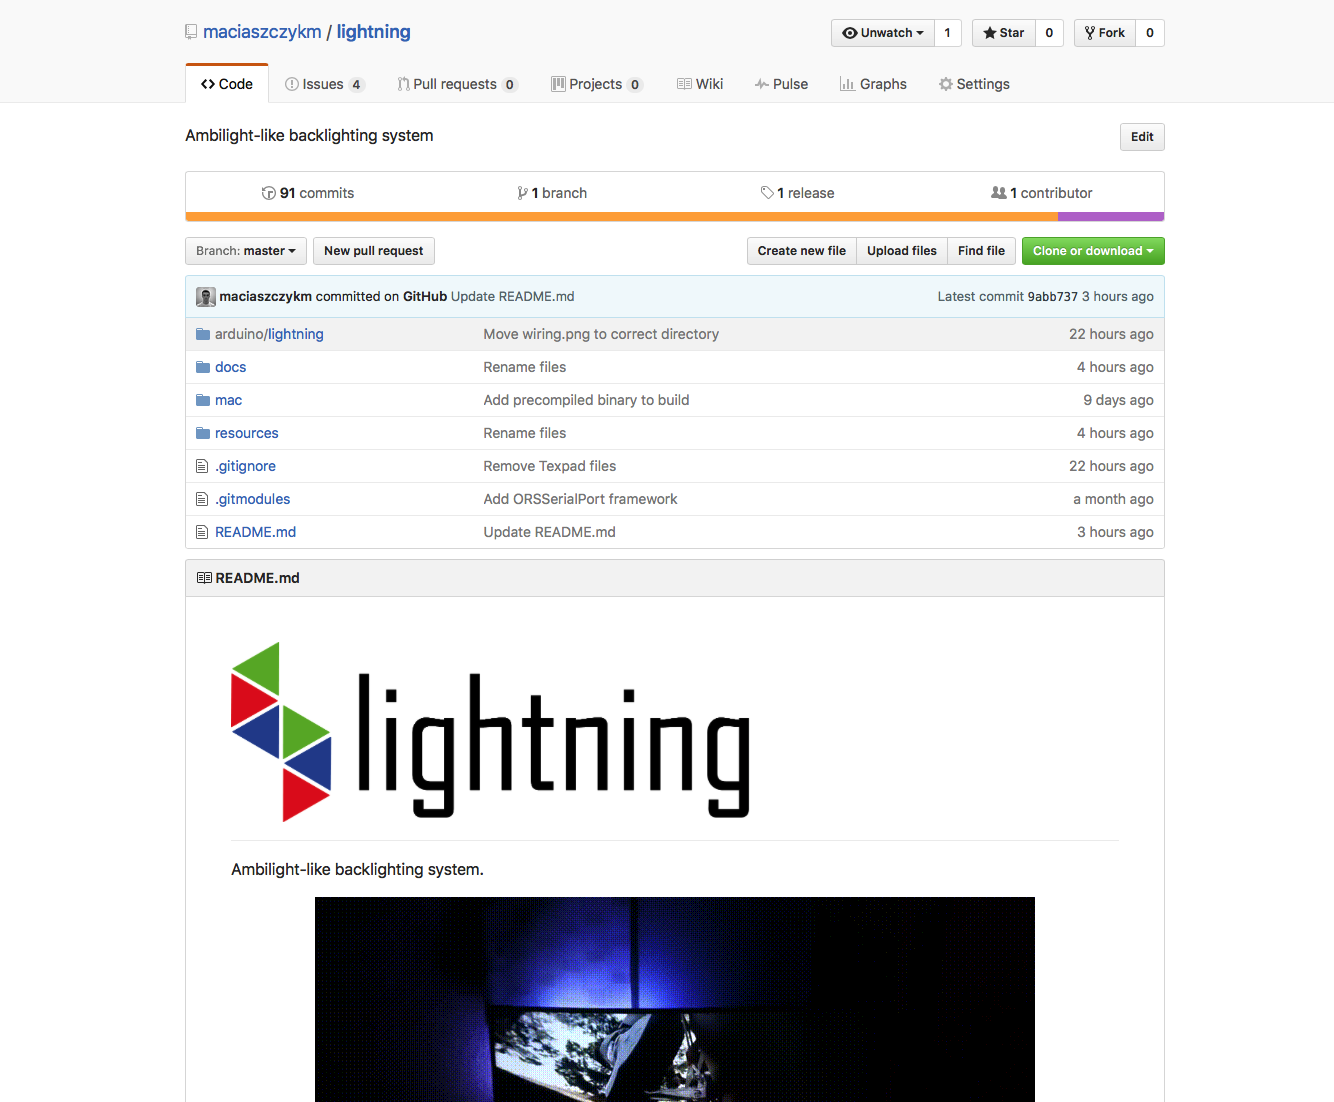
\includegraphics[width=\textwidth]{../resources/github.png}
\caption{Zrzut ekranu z repozytorium projektu}
\label{schemat}
\end{figure}

\subsection{Wykorzystane technologie}

Oprogramowanie mikrokontrolera zostało napisane w języku Arduino i to właśnie na tę platformę jest przeznaczone. Do jego napisania użyta została jedynie wbudowana biblioteka do obsługi portu szeregowego. Wykorzystano środowisko programistyczne Arduino \cite{arduinoide}.

Aplikacja sterująca została napisana w języku Swift, do stworzenia interfejsu graficznego wykorzystano framework\footnote{~Szkielet budowy aplikacji. Definiuje strukturę aplikacji oraz jej ogólny mechanizm działania, dostarcza zestaw komponentów i bibliotek ogólnego przeznaczenia do wykonywania określonych zadań.} Cocoa. Ponadto wykorzystano bibliotekę\\ORSSerialPort ułatwiającą komunikację poprzez port szeregowy \cite{orsserialport}. Wykorzystano środowisko programistyczne Xcode \cite{xcode}.

\subsection{Diagram klas}

% TODO

\subsection{Wzorce projektowe}

% TODO

\subsection{Interfejs użytkownika}

Interfejs, w tym przypadku graficzny, należy do elementów na które użytkownicy zwracają uwagę na samym początku, dlatego też powinien być on zaprojektowany z pomysłem i umożliwiać jak najprostsze poruszanie się po aplikacji.
Aplikacja posiada dwa tryby działania oraz tryb konfiguracji, dlatego też logiczny jest podział na trzy widoki przedstawione poniżej:

\begin{figure}[h!]
\centering
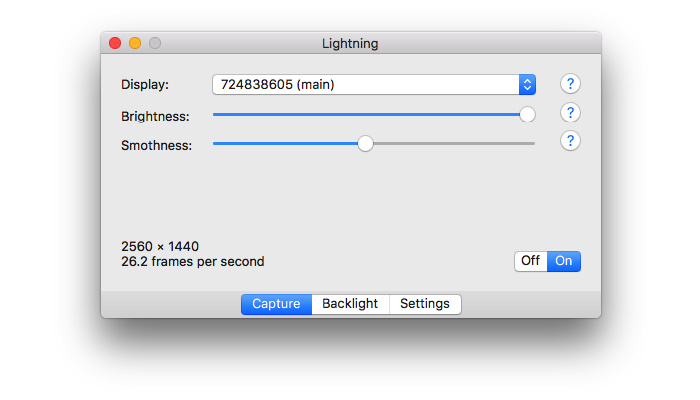
\includegraphics[width=\textwidth]{../resources/capture.png}
\caption{Widok trybu przechwytywania}
\end{figure}

\begin{figure}[h!]
\centering
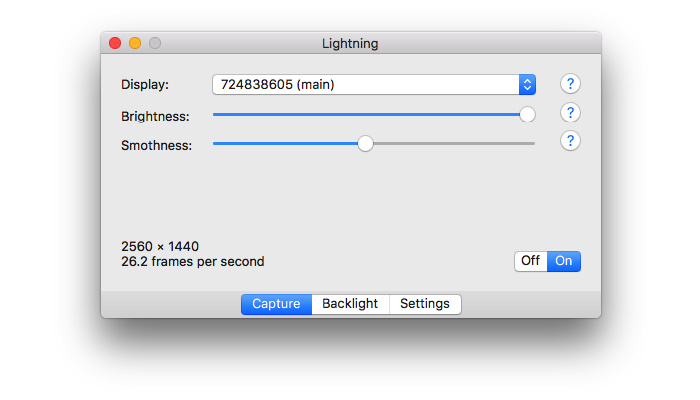
\includegraphics[width=\textwidth]{../resources/capture.png}
\caption{Widok trybu animacji}
\end{figure}

\begin{figure}[h!]
\centering
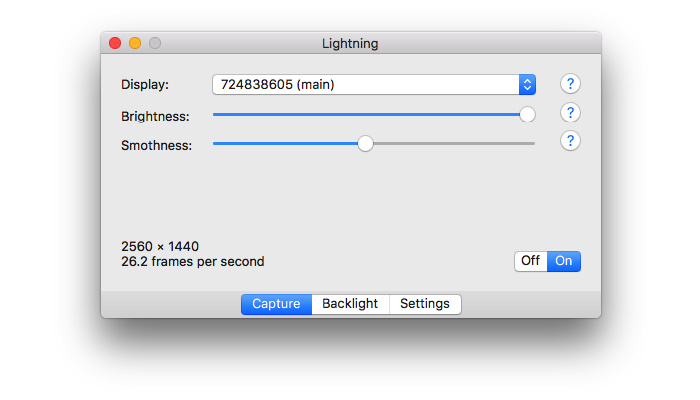
\includegraphics[width=\textwidth]{../resources/capture.png}
\caption{Widok konfiguracji}
\end{figure}

\vfill
\clearpage

% TODO

\section{Implementacja}

\subsection{Oprogramowanie mikrokontrolera}

Oprogramowanie mikrokontrolera napisane w natywnym języku Arduino mieści się w jednym pliku przedstawionym na listingu \ref{ino}.

\lstinputlisting[style=customarduino,caption=Kod oprogramowania mikrokontrolera]{../arduino/lightning/lightning.ino} \label{ino}

Tak jak to zostało wcześniej wspomniane celem mikrokontrolera jest odbieranie sygnału portem szeregowym i zapalanie diod w odpowiedniej konfiguracji. Wszystko musi odbywać się możliwie szybko, tak aby diody swój kolor zmieniały płynnie i nie pojawiały się żadne opóźnienia.

Pierwszym przyjętym założeniem jest odpowiednie formatowanie pakietów danych, które będą wysyłane przez port szeregowy. Aby żadne dane nie zostały utracone każdy pakiet musi składać się z nagłówka i danych właściwych. Nagłówki składają się z 11 bajtów, długość całego pakietu jest natomiast uzależniona od ilości diod zdefiniowanej w nagłówku:

\begin{itemize}
	\item Pierwsze 9 bajtów -- Zakodowana nazwa projektu, a więc "Lightning" jako tablica znaków.
	\item 10 bajt -- Liczba diod wykorzystywana przez użytkownika.
	\item 11 bajt -- Suma kontrolna nagłówka, czyli wartość 10 bajta XOR\footnote{~Alternatywa wykluczająca (z ang. exclusive or).} 0x13. W przypadku niezgodności wartości, pakiet zostaje pominięty przez mikrokontroler.
	\item Od 12 bajta -- Zakodowane kolory diod, na które mikrokontroler musi je zaświecić. Na każdą diodę przypadają 3 bajty danych:
	\begin{itemize}
		\item 1 bajt -- Wartość koloru czerwonego w skali od 0 do 255.
		\item 2 bajt -- Wartość koloru zielonego w skali od 0 do 255.
		\item 3 bajt -- Wartość koloru niebieskiego w skali od 0 do 255.
	\end{itemize}
\end{itemize}

Jeśli użytkownik korzysta z 25 diod, pakiety danych będą miały długość 86 bajtów, co jest małą liczbą biorąc pod uwagę zakładaną prędkość 115200 bitów na sekundę jeśli chodzi o transmisję portem szeregowym. Kluczem dla płynności działania aplikacji okazuje się więc odczyt i sprawne przekazanie instrukcji diodom.

% TODO opis oczekiwania na zmiany stanow etc.

\subsection{Aplikacja przeznaczona na komputer}

% TODO

\section{Podręcznik użytkownika}

Odpowiedzi na poniższe pytania mają za zadanie przybliżyć potencjalnym użytkownikom czym jest Lightning, co oferuje, jak działa i jak mogą oni zacząć z niego korzystać. Jest to skrót informacji pojawiających się w niniejszej pracy.

\subsubsection{Czym jest Lightning?}

Lightning jest systemem oświetlenia posiadającym podobną funkcjonalność jak technologia Philips Ambilight, a więc rozszerzanie obrazu wyświetlanego na ekranie na jego otoczenie za pomocą diod elektroluminescencyjnych.

\subsubsection{Jak działa Lightning?}

Lightning składa się z kilku komponentów, poza komputerem podłączonym do wyświetlacza niezbędny jest mikrokontroler Arduino Uno oraz taśma diod elektroluminescencyjnych\footnote{~Wszystkie komponenty systemu zostały wyszczególnione w rozdziale \ref{komp}}. Działanie systemu opiera się na przechwytywaniu obrazu z komputera z systemem macOS, uśrednianiem kolorów występujących w sferach na które podzielony został ekran\footnote{~Każda ze sfer odpowiada jednej diodzie.} i przesyłaniu informacji do mikrokontrolera. Jego zadaniem jest odbieranie informacji na temat kolorów diod i sterowanie diodami. System jest w pełni niezależny od wykorzystywanego wyświetlacza.

\subsubsection{Ile diód można podłączyć do Lightning?}

Do 255 diod, wystarczy to do oświetlenia powierzchni nawet za największym ekranem i zapewni uzyskanie wysokiej płynności działania nawet ze starszymi komputerami Mac.

\subsubsection{Jak zacząć korzystać z Lightning?}

Pierwszym etapem powinno być skompletowanie wszystkich komponentów systemu wymienionych w rozdziale \ref{komp}. Następnie należy je ze sobą podłączyć tak jak przedstawia to rysunek \ref{schemat}. Ostatnim krokiem jest wgranie oprogramowania na Arduino -- najłatwiej zrobić to za pomocą środowiska programistycznego Arduino, a także uruchomienie aplikacji sterującej na komputerze Mac. 

\subsubsection{Jak dodać własne animacje?}

Proces dodawania własnych animacji został opisany w rozdziale  \ref{animacje}.

\section{Przykładowa implementacja animacji} \label{animacje}

Tryb animacji udostępnia kilka podstawowych animacji, które po uruchomieniu wyświetlane są za pomocą diod. W celu dodania nowej animacji wystarczy dodać do projektu nową klasę na wzór klasy Disco przedstawionej na listingu \ref{anim} oraz zarejestrować ją w klasie Animations przedstawionej na listingu \ref{anims}

\lstinputlisting[style=customswift,caption=Klasa implementująca animację]{../resources/animation.swift} \label{anim}

Każda implementacja animacji musi implementować protokół Animation co wiąże się z koniecznością implementacji następujących metod:

\begin{itemize}
	\item setup(colors) -- Metoda ta uruchamiana jest jednokrotnie przy starcie animacji. Jej zadaniem jest odpowiednie zainicjalizowanie wszystkich diod. Kolory wybrane przez użytkownika przekazane są w parametrze.
	\item run(colors) -- Metoda ta uruchamiana jest przy każdym obiegu pętli w której odbywa się animacja. Jej głównym zadaniem jest przechodzenie pomiędzy kolejnymi stanami animacji. Kolory wybrane przez użytkownika przekazane są w parametrze.
\end{itemize}

Ponadto klasa animacji powinna roszerzać klasę LightController, która zawiera wszystkie podstawowe funkcje umożliwiające sterowanie diodami.

Animacja przedstawiona na listingu \ref{anim} inicjalizuje wszystkie diody na pierwszy kolor wybrany przez użytkownika, a potem w każdym następnym kroku zmienia kolor na kolejny i przesyła dane do mikrokontrolera.

\lstinputlisting[style=customswift,caption=Klasa służąca do rejestrowania animacji]{../resources/animations.swift} \label{anims}

Powyższy przykład obrazuje niski poziom skomplikowania implementacji nowych animacji.

\section{Analiza projektu}

W rozdziale \ref{kryt} zostały zdefiniowane kryteria analizy której poddane zostały istnie\-jące już systemy oświetlenia. Teraz biorąc pod uwagę te same kryteria zostanie przeanalizowany Lightning.

\begin{figure}[h]
\centering

\includegraphics[width=\textwidth]{../resources/logo.png}
\caption{Logo Lightning}
\end{figure}

\begin{table}[h]
\centering
\begin{tabular}{| l | l |} 
\hline 
Koszt & 316,70 zł\footnote{~Kwota ta mogłaby ulec znacznemu zmniejszeniu w przypadku wykorzystania dostępnych zamienników dla mikrokontrolera Arduino Uno a także taśmy diod elektroluminescencyjnych, tak jak zostało to opisane w rozdziale \ref{komp}.}\\ \hline
Rodzaj systemu & do samodzielnego montażu, \\ \hline
& zewnętrzny \\ \hline
Płynność działania & bardzo wysoka \\ \hline
Możliwość konfiguracji & średnia  \\ \hline
Interfejs użytkownika & intuicyjny  \\ \hline
Dodatkowe możliwości &  tryb animacji, duża rozszerzalność \\ \hline
Wspierany sprzęt i oprogramowanie &  komputery z systemem macOS  \\ \hline
Licencja & kod otwartoźródłowy  \\ \hline
\end{tabular} 
\caption{Analiza systemu oświetlenia Lightning}
\end{table}

% TODO zdjęcia gotowego projektu

Do niewątpliwych zalet Ligthning należy z pewnością niski koszt, otwartożródłowy kod i łatwa rozszerzalność systemu. Użytkownicy znający podstawy programowania mogą z łątwością dopasować projekt do swoich potrzeb, nie jest to jednak konieczne ponieważ większość opcji konfiguracyjnych jest już dostępna. Ciekawym dodatkiem jest tryb animacji. Animacje można dodawać według własnych upodobań. Dodatkowo system można podłączyć do dowolnego wyświetlacza połączonego z komputerem.

Podobnie jak w przypadku wszystkich innych analizowanych rozwiązań poza technologią Philips Ambilight Ligtning jest zewnętrznym systemem oświetlenia co wiąże się z koniecznością podłączenia dodatkowych urządzeń do wyświetlacza. Kolejną z wad jest przeznaczenie na komputery z systemem macOS, jest to związane z chęcią uzyskania jak najwyższej płynności działania.

\section{Perspektywy rozwoju projektu} \label{prp}

W celu dalszego rozwoju stworzonego systemu oświetlenia należy rozważyć wprowadzenie następujących usprawnień:

\begin{itemize}
	\item Zaawansowana konfiguracja ułożenia diod -- Obecnie diody rozmieszczane są równomiernie na górnej i bocznych krawędziach. Wprowadzenie trybu konfiguracji w którym istniałaby możliwość dopasowania każdego obszaru przechwytywania osobno byłoby znacznym usprawnieniem.
	\item Korekcja kolorów -- Obecny stan systemu umożliwia kontrolę jasności diod oraz wygładzania przejść pomiędzy kolejnymi stanami. Wprowadzenie korekcji kolorów umożliwiłoby dopasowanie koloru diod do otoczenia, czyli na przykład czerwonej ściany za wyświetlaczem.
	\item Częstotliwość przechwytywania -- Poza korekcją kolorów kolejnym wartościowym dodatkiem byłoby wprowadzenie ograniczenia częstotliwości przechwytywania.
	\item Poprawki graficzne szaty graficznej -- Dodanie ikony dla aplikacji sterującej, użycie obrazka wyświetlacza trybie konfiguracji czy też wyświetlanie poglądu animacji.
	\item Automatyczne testy -- Automatyczne budowanie i testowanie całej aplikacji przy każdej zmianie podniosłoby jakość projektu. 
\end{itemize}

\chapter{Podsumowanie}

\section{Dyskusja wyników}

Przejście przez kolejne fazy tworzenia oprogramowania, od postawienia wymagań, przez zaprojektowanie, zaimplementowanie aż do stworzenia dokumentacji umożliwiło stworzenie systemu oświetlenia, który stanowi konkurencyjną alternatywę dla istniejących już rozwiązań.  Lightning udostępnia w pełni funkcjonalny tryb przechwytywania ekranu, tryb animacji, posiada możliwości konfiguracyjne, działa płynnie a koszt jego konstrukcji jest najmniejszy spośród wszystkich analizowanych systemów oświetlenia.

Poza osiągnięciem rezultatu w postaci gotowego systemu oświetlenia, w niniejszej pracy autorowi udało się zgromadzić użyteczne informacje dotyczące tematyki tworzenia oprogramowania przeznaczonego na mikrokontrolery, komunikacji portem szeregowym czy też zagadnieniom dotyczącym efektywnego przechwytywania obrazu.

\section{Perspektywy rozwoju pracy}

W celu dalszego rozwoju niniejszej pracy należy rozważyć przede wszystkim dalsze prace nad stworzonym systemem oświetlenia. W rozdziale \ref{prp} przedstawione zostały liczne możliwości rozwoju projektu, ich realizacja byłaby z pewnością sporym krokiem w przód. Podjęcie się tego zadania oznaczałoby jednak trzymanie się obecnej tematyki pracy, a przecież wykorzystanie mikrokontrolerów podłączonych do komputera nie jest jedynym możliwym rozwiązaniem. 

Odejście od obecnej tematyki pracy zostałoby zapewnione poprzez stworzenie oprogramowania przeznaczonego bezpośrednio dla telewizorów. Aplikacja steru\-jąca mogłaby wtedy zostać przeniesiona na urządzenia mobilne. W tym przypadku wymagane byłoby dokładne zapoznanie się z dostępnym sprzętem i istniejącymi ograniczeniami. Z pewnością jednak takie rozwiązanie spotkałoby się z szerokim gronem odbiorców.

Rozwiązaniem pośrednim byłoby przeniesienie oprogramowania przechytującego obraz do mikrokontrolera o większej mocy obliczeniowej, na przykład Raspberry Pi. W tym przypadku sterowanie diodami jak i przechytywanie obrazu mogłoby się odbywać bezpośrednio na nim. Mikrokontroler mógłby samodzielnie odtwarzać filmy bez konieczności podłączania kompuera.

\addcontentsline{toc}{chapter}{Bibliografia}
\begin{thebibliography}{99}
\bibitem{czasprzedtv} {\tt http://www.wirtualnemedia.pl/artykul/coraz-dluzej-ogladamy\-telewizje-najwiecej-czasu-przed-szklanym-ekranem-spedzaja\--seniorzy-raport}.\\Data dostępu -- 20.01.2017.
\bibitem{diagramoko} {\tt https://www.indiegogo.com/projects/lightpack-2-light\-orchestra-for-your-living-room-tv-videogames}. \\Data dostępu -- 20.02.2017.
\bibitem{ambilightaoko} {\tt http://www.embedded.com/print/4012996}. \\Data dostępu -- 20.02.2017.
\bibitem{ambilight2} {\tt http://www.komputerswiat.pl/media/2016/224/4688581/003\-philips-ambilight-2-sides.jpg}. \\Data dostępu -- 06.02.2017.
\bibitem{swiftpub} {\tt https://swift.org/documentation/TheSwiftProgrammingLanguage\-(Swift3.1).epub}. \\Data dostępu -- 20.02.2017.
\bibitem{swiftdev} {\tt https://itunes.apple.com/us/book/app-development-with-swift/\-id1118575552?mt=11}. \\Data dostępu -- 20.02.2017.
\bibitem{swiftstr} {\tt https://swift.org}. \\Data dostępu -- 20.02.2017.
\bibitem{swiftapple} {\tt https://developer.apple.com/swift/}. \\Data dostępu -- 20.02.2017.

\bibitem{diody} {\tt https://botland.com.pl/lancuchy-i-matryce-led/2443-lacuch\-led-rgb-12-mm-ws2801-cyfrowy-adresowany-25-szt.html}.\\Data dostępu -- 17.01.2017.
\bibitem{zasilacz} {\tt https://botland.com.pl/zasilacze-sieciowe-5-v/1364-zasilacz\-impulsowy-5v-25a-wtyk-dc-55-21-mm.html}.\\Data dostępu -- 17.01.2017.
\bibitem{wtyk} {\tt https://botland.com.pl/szybkozlacza/1590-wtyk-dc-55-x-21\-mm-z-szybkozlaczem.html}.\\Data dostępu -- 17.01.2017.
\bibitem{arduino} {\tt https://botland.com.pl/arduino-moduly-glowne/1060-arduino\-uno-r3.html}.\\Data dostępu -- 17.01.2017.
\bibitem{usb} {\tt https://botland.com.pl/przewody-usb-a-b-20/5313-przewod\-usb-a-b-tracer-18m.html}.\\Data dostępu -- 17.01.2017.
\bibitem{schemat} {\tt https://cdn-learn.adafruit.com/assets/assets/000/001/484/\-medium800/led\_pixels\_wiring-diagram.png?1396773276}.\\Data dostępu -- 17.01.2017.
\bibitem{github} {\tt https://github.com/maciaszczykm/lightning}.\\Data dostępu -- 17.01.2017.
\bibitem{arduinoide} {\tt https://www.arduino.cc/en/main/software}.\\Data dostępu -- 18.01.2017.
\bibitem{orsserialport} {\tt https://github.com/armadsen/ORSSerialPort}.\\Data dostępu -- 18.01.2017.
\bibitem{xcode} {\tt https://developer.apple.com/xcode/}.\\Data dostępu -- 18.01.2017.
\bibitem{ambilight} {\tt http://www.cobra.fr/media/wysiwyg/logo-ambilight.jpg}. \\Data dostępu -- 06.02.2017.
\bibitem{lpk} {\tt https://www.kickstarter.com/projects/woodenshark/lightpack\-ambient-backlight-for-your-displays}. \\Data dostępu -- 09.02.2017.
\bibitem{lps} {\tt http://lightpack.tv/}. \\Data dostępu -- 09.02.2017.
\bibitem{legacy} {\tt https://github.com/Atarity/Lightpack}. \\Data dostępu -- 09.02.2017.
\bibitem{lp2k} {\tt https://www.kickstarter.com/projects/woodenshark/lightpack\-2-ultimate-light-orchestra-for-your-livi}. \\Data dostępu -- 09.02.2017.
\bibitem{lp2s} {\tt http://lightpack.tv/promo/index.php}. \\Data dostępu -- 09.02.2017.

\end{thebibliography}

\addcontentsline{toc}{chapter}{Spis rysunków} 
\listoffigures

\addcontentsline{toc}{chapter}{Spis tabel} 
\listoftables

\addcontentsline{toc}{chapter}{Spis listingów} 
\lstlistoflistings

\end{document}